\pdfbookmark[0]{Writing and formatting guide for your thesis}{Writing and formatting guide for your thesis}
\setcounter{chapter}{-1}
\chapter{Writing and formatting guide for your thesis}
%\pagestyle{plain} 


\vspace{-3mm}
Dear colleague,

\textit{Scientific writing} is the number one skill of a successful scientist. Mastering this proficiency requires extensive practice, iteration, and feedback. To support you in the first steps to master this essential skill, we provide you with a summary of the essential style rule and some writing style guidelines. We are happy that you are taking those first steps on this demanding but exciting journey with us. 


\vspace{-3mm}
%\noindent
\begin{flushright}
Success in writing your thesis, \\
Your thesis advisers at IGAM\\
\end{flushright}

\noindent \physit{The following notes were written by Paul Beck,\,PhD,  with addenda by the teachers and advisers at IGAM. (Living document, Version: April 2021)\footnote{Comments or feedback on the IGAM thesis template should be directed to \href{mailto:paul.beck@uni-graz.at}{paul.beck@uni-graz.at}.}}


\vspace{-5mm}
\section*{Writing}
\noindent
The language has to be clear and objective. Science requires quantifying things and putting results into context. The following items will give you a first impression of where to be on your toes.
\begin{itemize}
    \item  Avoid qualitative adjectives (e.g., very, a lot, little, many) and refrain from expressing personal beliefs or using sarcasm. Following the maxim of \textit{'show, don't tell'} a sentence like \textit{'Sample A is much better than sample B'} should be rewritten into something like \textit{'The statistical uncertainty of the measurements of parameter X in sample A is three times smaller than in sample B.'}
    
    \item Consider your \textit{'Why?'}. A sentence like \textit{'Studying stars is important'}, is a general statement which says everything and nothing at once. Following the principle,  \textit{Show, don't tell} you can implicitly show \textit{why} something has significance, rather than saying so, \textit{'Stars are the building blocks of the galaxy. Studying these objects allows for a better understanding of how our milky way evolved'.}
    
    \item Avoid wordy sentences. A typical sentence should be less than two full lines. A good trick is to mark each sentence longer than that with a text marker on a printout.  Then split such sentences into two or three shorter sentences.
    
    \item Write in an active form. For example, write \textit{`Galileo has found 4 Jovian satellites'} instead of \textit{`The four Jovian satellites have been found by Galileo'}. The active form will help you write more precise and shorter sentences. Remember that your text may need to be read and understood by people with lower language skills than yours. Make the reader's life easier.

    \item Use abbreviations sparsely and only for your most important phrases or key terms. At first use in the text body, they need to be defined. The use of abbreviations or acronyms is highly de-appreciated by editors in a paper's title and abstract. Consequently, colloquially used acronyms, such as HRD, RV, ZAMS, or TAMS, need to be spelled out in the title and abstract. 

    \item Similar applies for each mathematical symbol used in the text and equation must be defined at first use $-$ an occasional reminder of the meaning throughout the paper doesn't hurt. 
    
    \item Only use footnotes to indicate webpage links, e.g., for MESA, \textsc{Phoebe}, AstroPy, data catalogs portals, or as demonstrated above for a specific document of high relevance to your work.
    
    \item References to papers are fundamental for your work's scientific integrity and placing your work into the broader context of timely and relevant research. The examples below and in the next section and Chapter\,\ref{sec:intro} demonstrate the use of the implemented BibTex-package.
    
    \item Short notes on grammar. Always put a ``,'' before the word ``which'', but never before ``that''. Remember the ``s'' at the end of the verbs in the third singular person. If possible, try to keep the tenses of the verbs always the same throughout the text.  Write all numbers between zero and ten as a word while keeping the others in number.
    
    \item Plagiarism and doctoring the data are the cardinal sins of a scientist. Such behavior is not tolerated. Be aware of the automated plagiarism check during the submission process. If detected, we would consider this a major abuse of our trust in you and reserve the right to take academic action.
    
    %\item In a continued thought, refrain from starting follow-up sentences with 'This'.
\end{itemize}

%\vspace{5mm}
\subsection*{Additional self-study resources on scientific writing}
\begin{itemize}
    
\item The best way to improve your writing is to read much scientific literature. Different authors write differently, though, so you have to find your own style. You can do this by exercising your writing and reading and identifying authors who write in a way you like. Keep notes on the content of the papers you read. We also recommend reading the article on reading \hbox{papers by \cite{PaperOnRreadingPapers}.}
    
    \item Concise collections of lecture notes on the topic are available in the books by Prof. Arnold Hanslmeier\footnote{The PDF of the book (in German) is available at  \hbox{\href{https://bookboon.com/de/wissenschaftliches-arbeiten-ebook}{https://bookboon.com/de/wissenschaftliches-arbeiten-ebook}}} and \cite{Mack2018Book}\footnote{The PDF of the book (in English) is available at \href{https://spie.org/samples/9781510619142.pdf}{https://spie.org/samples/9781510619142.pdf}}.
    
    \item You may use modern software, such as \href{http://www.Grammerly.com}{Grammerly.com}, to check your thesis's grammar and spelling. Doing so allows us to focus on discussing science and content and streamline the iteration process.
    
    \item Play around with \LaTeX. Writing in this scripting language will become second nature to you. You are encouraged to search \LaTeX-documentation and advance your thesis beyond this template, e.g., defining your own frequently used symbol-groups. A good source of documentation about working with \LaTeX\ is provided by Overleaf: \href{https://www.overleaf.com/learn}{https://www.overleaf.com/learn}.
    
    Commented text, using '\%' allows you to keep hidden notes. This is particular helpful to keep  notes or an earlier version of a sentences or paragraph, you wanted to reword.  
    % While they are not shown in the text of the PDF, they are still part of the file and can be read out. There are twitter accounts, which echo the funniest or most embarrasing hidden coments from papers on the preprint server ArXiv: e.g. @LeaksPh is eavesdropping on tex-source comments in papers posted to astro-ph.
    Use colors to mark action items or text during the iteration phase. Some examples are shown at the end of this chapter.
\end{itemize}

A very common mistake beginners make is to write meaningless sentences. This happens because you know well what you want to say, write it down in a sentence in a meaningless way due to lack of practice.  Yet, because you know what you want to say, the sentence you have just written looks useful to you. There is a straightforward strategy that you should apply to avoid this. Write a piece of text, then read it aloud or (even better) record it, and finally listen to it, trying to understand what you want to say from listening to what you read. If you cannot understand the meaning of what you said, then there is something wrong with that text.

A final piece of advice. Write something, then leave it aside without reading it for a few days and then returning to it. The more times you do this process, the better the text will become.



%\newpage
\section*{Elements of a scientific work}
\noindent
In general, the style in this thesis template follows the formatting guidelines\footnote{The PDF version of the editorial guidelines: \href{https://www.aanda.org/doc_journal/instructions/aadoc.pdf}{https://www.aanda.org/doc\_journal/instructions/aadoc.pdf} \label{fn:AAstyleGuide}} of \physit{Astronomy \& Astrophysics {\rmfamily (A\&A)}}, the European  workhorse journal for astrophysics. The only divergence from these guidelines is the more extensive bibliographic information of cited papers and how you can \hbox{present your programming code in the appendix.}

Below, we summarize the essential guidelines to follow in your writing. 
Examples for typical elements, such as including citations, cross references, and the inclusion of figures and tables are shown in Chapter\,\ref{sec:intro} and Chapter\,\ref{sec:data}. Each content element (e.g. abstract, table of contents, chapter, bibliography) starts on the right page (recto). This means that in some cases the left side (verso) will be left blank. \LaTeX\ will take care of this.





\subsection*{Structure of your thesis}
\begin{itemize}
    \item \physbf{Abstract:} It follows the structured abstract of A\&A. Write a few sentences for each of the indicated blocks. The length of the abstract should be about half a page. Do not use abbreviations, acronyms, or formulae in this block.  Typically this section is written as last.

    \item \physbf{Acknowledgements:} This section allows you to give explicit credit to people, institutions, programs, or projects. This template shows typical examples. Many telescopes, space missions or software projects provide predefined sentences for the acknowledgements which you simply should copy. Make sure that you \hbox{cite the requested instrumental-reference papers in the text body.}
    
    \item \physbf{Text body:} consists of the main content of the paper. It starts with the first chapter, the \physit{Introduction}, where you explain, how your research question connects to the bigger picture  of the field. Do not write a review on the whole field. Rather follow the recipe depicted in \Fig{fig:logicalFlow}. Ideally, you pick up the argumentative thread again in the the final section on \physit{Discussions \& Conclusions} and demonstrate how your work has advanced on the addressed topics.
    
    \item  Name and content of the following chapters are not defined. However, it should loosely follow the logic: \physit{Methodology}, \physit{Observing techniques} (or simply) \physit{Data $-$ Analysis $-$ Results $-$ Discussions \& Conclusions.} Optimally, you have a \LaTeX\  file per chapter, as demonstrated in this template.
    
    \item Sections or subsections will follow the logic of your work. Use lower case for all words in chapter and section title headings, except for the first character. Do not introduce subsubsections.
    

    
    \item \physbf{Bibliography:} This section provides all information to find and retrieve your cited literature unambiguously. If you are using the recommended BibTex package to manage your references, this part will be taken care of for you by \LaTeX. How to work with BibTex is demonstrated below.
    
    \item \physbf{Appendix} is used to place extensive content, which would otherwise interrupt the reader. It can have several sections, labeled with capital letters. You typically would place code, additional figures, or large tables. Content in the appendix, such as figures, tables, or supplementary method descriptions in sections, needs to be referenced at least once in the main text body.
    
    \item For a master or PhD thesis, include the \physbf{Curriculum Vitae}. Complete the predefined sections. List what is relevant to your studies and research activity.
    
    \item List your scientific publications in the \physbf{List of publications}.
    
\end{itemize}

\begin{figure}
    \centering
    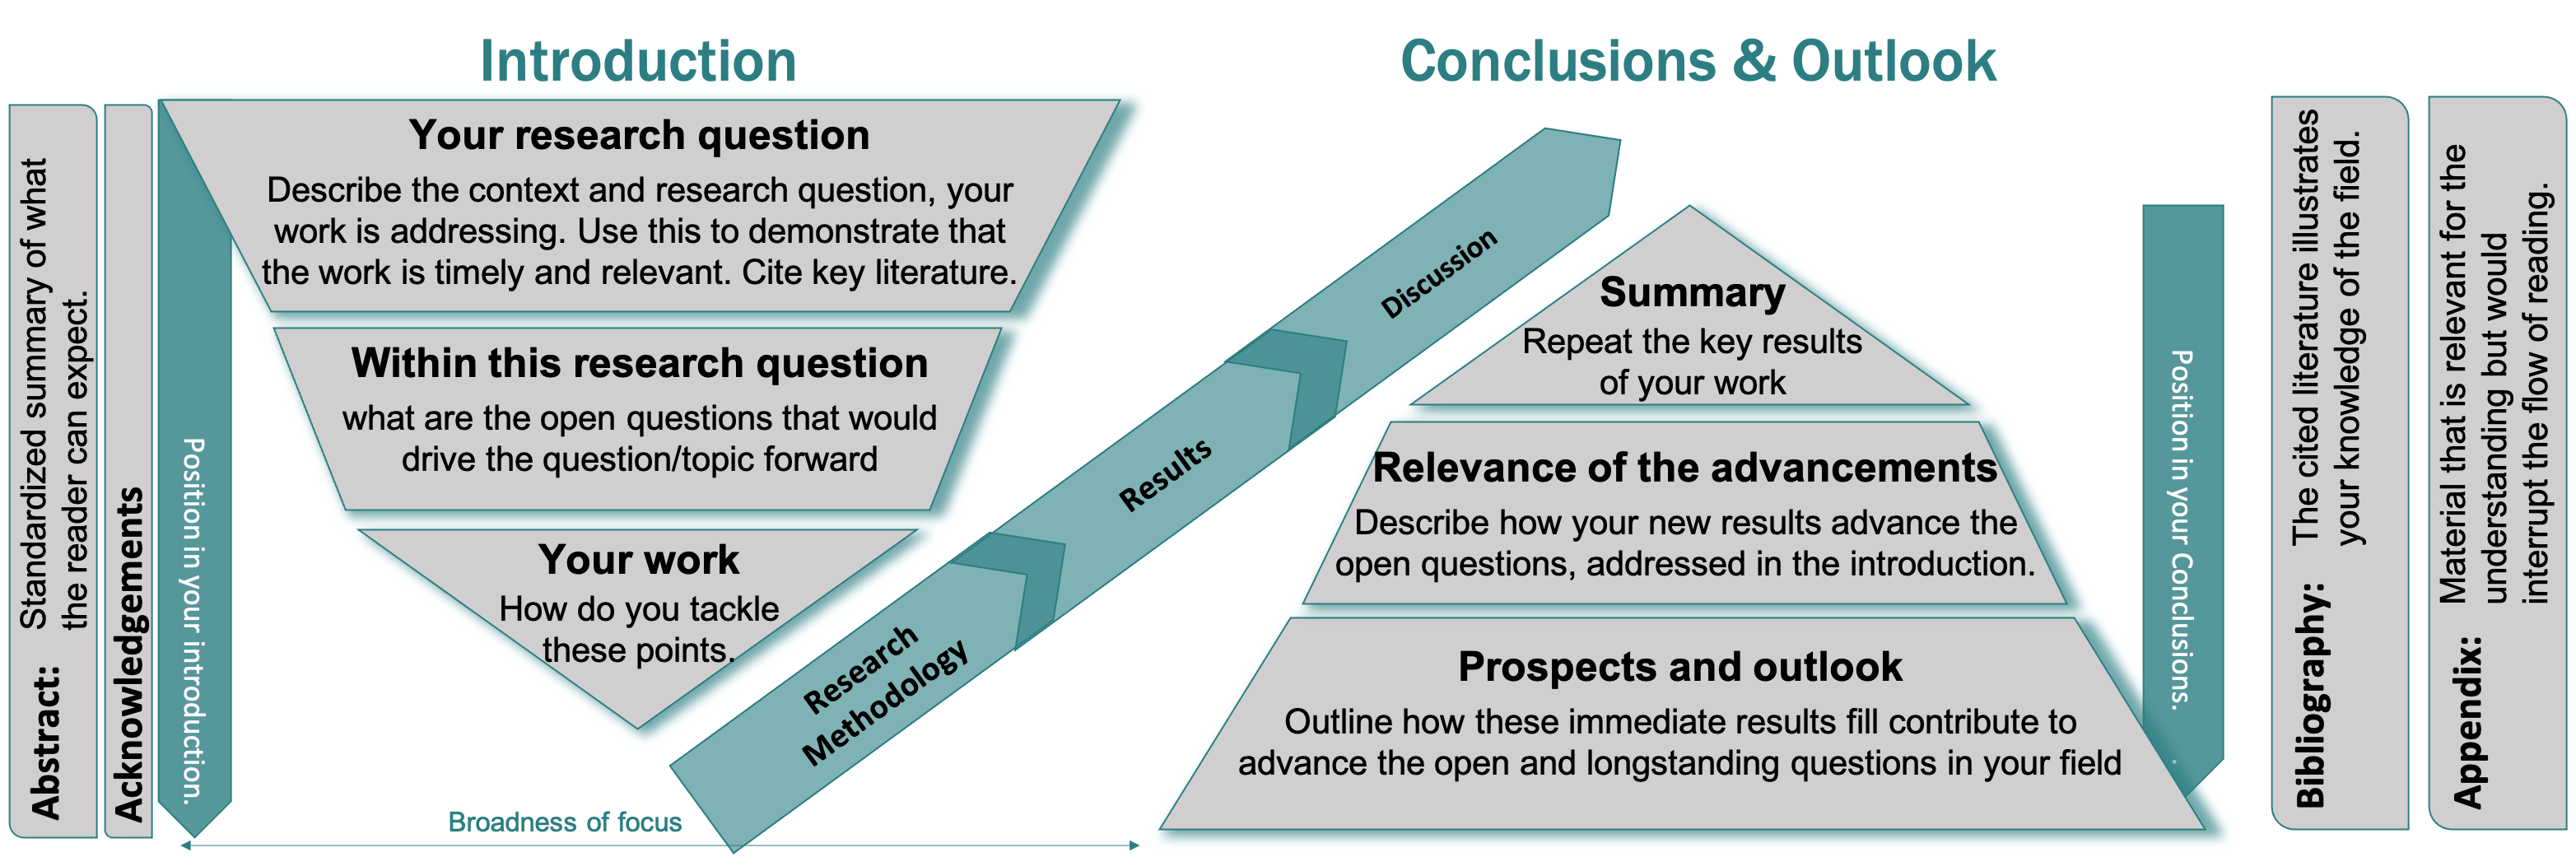
\includegraphics[width=\textwidth]{gfx/constructionMap.png}
    \caption{Schematic structure of the elements of a thesis or research paper. The cones depict the ideal logical flow of the chapters of the \textit{Introduction} and \textit{Conclusions \& Outlook}. }
    \label{fig:logicalFlow}
\end{figure}

%The logical flow of a thesis is illustrated in \Fig{fig:logicalFlow}.
As the first step in your writing process, we recommend that you lay out the anticipated structure and approximate content by crafting chapter and perhaps the main section titles. This first structure can already be implemented in the template and be discussed with your adviser early on. Doing this will allow you to have a more straightforward path to assess the thesis's content and expected workload.


\subsection*{Literature references \& managing your bibliography}
\begin{itemize}
    \item A citation is needed whenever a bibliographic reference to published content is required. The leading astronomical journals use the style of inter-textual citations. In this format, you see the first author's name in the text, most likely to be followed by \textit{et al.} to indicate that more than two authors have signed the paper and the publication year of the paper. The \textit{Bibliography} section in the rear provides all the information on how to retrieve the cited article. Each item listed in the bibliography needs to \hbox{be referenced at least once in the paper.}
    
    \item BibTex is a powerful software package that will help you to easily manage your bibliographic references and the respective bibliography. By using the citation commands 
    $\backslash$cite\{\}, 
    $\backslash$citep\{\}, 
    $\backslash$citep[]$\{\}$, and 
    $\backslash$citep[][]\{\} you create inter-textual references. The following examples show how the above mentioned macros can be used in the syntax of a sentence: 


    
     $-$ \textit{It was shown by \cite{Beck2015} that the long-periodic variations of the radial-velocity signal of $\theta^1$\,Tau originates from stellar activity.} \\
     $-$ \textit{Combining remote-sensing image data with in-situ measurements have lead to an improved flare-CME characterization 
     \citep{Temmer2017}.}\\
     $-$ \textit{The extreme-ultraviolet Radiation from A-stars has significant implications for the formation of \citep[and references therein]{Fossati2018}.}\\
     $-$ \textit{This topic has been discussed in the recent literature
    \citep[e.g. see][and references therein]{Hanslmeier2018phsabook,Veronig2020}.}
    
    \item To cite from a monography use the $\backslash$citep[]\{\} command to reference the book you are citing. If of relevance you can note to which chapter or page you are referring to in the squared brackets of the makro.

    \item Those macros access the content of the file \textit{bib-refs.bib}. To add references, copy the content from \textit{'export citation'} on the NASA ADS webpage of a paper into the bib-file. Experience has shown that it will improve the readability of your  \LaTeX\ code if you change the predefined bibcode (e.g., 2017SoPh..292...93T) into a more user-friendly keyword (e.g., Temmer2017), which is then used in the macros mentioned above to cite the paper.

\end{itemize}

\subsection*{Cross references to elements inside your thesis}
\begin{itemize}
    \item Each Figure, Table, and Equation presented in the paper needs to be referenced at least once in the text body. The objects of each group (figures, tables, equations) must be introduced in the paper in consecutive order: Reference Fig.\,1 in the text before you mention Fig.\,2.
    
    \item Abbreviate the following expressions unless they appear at the beginning of a sentence:  \textit{Sect., Sects., Fig., Figs., Col., Cols.}. \textit{Table} and \textit{Listing} are never abbreviated in a paper. Write the object abbreviation in the upper case if used as a numbered reference. Otherwise, object names should not be abbreviated and written in lower case.
    
    $-$ \textit{\Figure{fig:singelPanelPlot} shows the position of 18 eccentric binary in the HR diagram.}\\
    $-$ \textit{As shown in \Fig{fig:singelPanelPlot}, the 18 eccentric binary are found on the low-luminosity red-giant branch (RGB).} \\
    $-$ \textit{The 18 eccentric binary are found on the low-luminosity RGB (see \Fig{fig:singelPanelPlot}).}
    
    \item To generate an automated numbering, you need to create a reference-able label, using \textit{$\backslash$label$\{$keyword$\}$}. Calling the keyword through the reference macro, \textit{$\backslash$ref$\{$keyword$\}$} will create the reference in the text. You can freely choose the keyword. Experience has shown that it is good practice to encode what kind of object you are referencing into the keyword, e.g.
    \textit{$\backslash$label$\{$fig:HRD$\}$}, 
    \textit{$\backslash$label$\{$tab:redGiantCatalogue$\}$}, 
    \textit{$\backslash$label$\{$eq:pythagoras$\}$}, or
    \textit{$\backslash$label$\{$sec:introduction$\}$}.

    Note that the template contains customized macros in the \textit{main.tex} for all full and abbreviate element names. This way, you only need to type, e.g. \textit{$\backslash$Fig\{fig:HRD\}}, instead of \textit{Fig.$\backslash$,$\backslash$ref\{fig:HRD\}}


\end{itemize}


%\newpage
\subsection*{Figures}
\noindent
Example of single and multi-panel figures and their caption format are given in Fig.\,\ref{fig:singelPanelPlot} and Fig.\,\ref{fig:multiPanelPlot}, respectively.
\begin{itemize}

    \item \physbf{Position:} to be placed on top of the page, using the figure attribute~\textit{[t!]}. Do not place a figure on the first page of a chapter.

    \item \physbf{Message:} be clear to yourself, what take away message is, which you want to give to the reader of your paper by showing this figure. Now optimize your figure to maximize the storytelling: use different symbols, line styles, and colors. A good test for a colored figure is if it is still readable on a black-and-white printout.

    \item \physbf{Caption}: The first sentence of the figure's caption should be a sentence describing the figure. This sentence should start without 'The' / 'This', 'A / An',  or similar.
    Describe all symbols and line styles used in the figure. Express no physical or scientific interpretation of the depicted context.
    
    \item Refer to the figure's axes as the \textit{'horizontal'} and the \textit{'vertical axes'}, instead of the x- and y-axis, respectively.
    
    \item For multi-panel figures, you should refer to the individual panels by using \textit{'top left panel'}, \textit{'middle bottom panel}, or \textit{'bottom right panel'}. 
    
    \item In case you show additional figures depicting different data but using the identical symbol and color scheme, you can refer to the first figure explaining the meaning. State something like \textit{'Meaning of the colors and symbols is similar to Fig.\,XY'}.
        
    \item If you show a figure previously published in another article, you need to indicate the source, such as \textit{(Figure taken from REFERENCE)}. In case somebody provided you  an unpublished figure, you would state  \textit{(Figure provided by PERSON).}    
    
    \item \physbf{Axis labels}: produce plots with readable axes, labels, and ticks. Unreadable labels are the easiest way of getting into \hbox{trouble with the referee (or adviser).}
    

    \item Format: preferably use PNG to avoid excessive file sizes for figures depicting many datapoints.
    

    
\end{itemize}

%\newpage
\subsection*{Tables}
\noindent
An example of a simple, complex and a multi-page table are given in Tab.\,\ref{tab:false_positives}, Tab.\,\ref{tab:asteroseismicValues}, and Tab.\,\ref{tab:longTable} respectively.

\begin{itemize}
    \item \physbf{Position:} to be placed on top of the page, using the table attribute~\textit{[t!]}. Do not place a table on the first page of a chapter.%(The only exception are tables depicting a code's functions, as shown in Appendix\,\ref{chap:appendixCode}.)
    
    \item \physbf{Caption:} (on top of the table): The table caption should be a one-line sentence, describing the table and placing it into the work or paper context. This sentence should start without 'The' / 'This', 'A / An', or similar.
    
    \item \physbf{Layout:} Tables start from above with a double vertical line, followed by the table header, followed by a single line, followed by the table's content. A final horizontal line is closing the table. 
    
    If appropriate, you can use horizontal lines in the table body to mark separations. In this case, the A\&A guidelines refer to the separated blocks as panels. An example is given in  Table\,\ref{tab:false_positives}.
    
    \item The content of the table is typically formatted to the left or right of the column. If you wish to do the extra work for a nice looking table, you can center the header, as shown in Tab.\,\ref{tab:asteroseismicValues}.

    \item \physbf{Tablefoot:} (text block below the actual table starting with \physbf{Notes.}) should contain all relevant information for each column should be provided in the table foot. If you use abbreviated references, you should give the connection to the inter-textual references here. Express no physical or scientific interpretation here. The tablefoot-macro requires an empty line between the text and the table to avoid layout issues.
    
    \item \physbf{Extensive tables} can be presented in the landscape format and / or be split over several pages (longtable). Consider placing it in the Appendix. In this case, you could place the tablefoot-block into the text body of the Appendix as demonstrated in Appendix\,\ref{chap:appendixExtensiveTables}
    
    \item Tables are usually not used in the Introduction or Conclusions chapter.
\end{itemize}

%\newpage
\subsection*{Equations}
\begin{itemize}
    \item Treat equations as part of the sentence and place them like a subordinate clause. See Eq.\,\ref{eq:pyth1}\,and\,\ref{eq:pyth2} for an example.

    \item All mathematical symbols used in the equation need to be defined near the equation, if not defined before in the text. Mention the physical units of the parameter used in the equation.
    
    \item Text in equations or math mode is written in italics per default. In case you want to place a subscript text, which is not an index, you need to force it to be non-italic, e.g., P$_{\mathrm{orb}}$.
    
    %\item multiple equations (if \&=\&, alingement of equations)
    
    %\item \ref{eq:pyth1}, \ref{eq:pyth2} 
\end{itemize}


\subsection*{Presentation of code and code snippets}

One of the bricks of the fundament of science is the replicability of disseminated results. Therefore, the modern standard of research journals that any elaborated code that is used for the data analysis presented in the paper should be made available to the reader. Such code is typically distributed on pages such as GitHub.com. 
For your thesis, we simulate such public distribution of code by presenting your code in the appendix. Discuss with your adviser if or what part of your code should be part of the thesis work. \Listing{code:tidalSettings} and Appendix\,\ref{chap:appendixCode} demonstrate how code (snippet) or pseudo-code is to be presented in the textbody and appendix your thesis, respectively.

\noindent
\physbf{\bfseries\sffamily Presentation in the text body}
\begin{itemize}
    \item Only essential code parts or concepts (via snippets or pseudo code, respectively) should be presented in the main body of your thesis. 
    
    \item The \texttt{verbatim} command is a very severe command, which cannot be used within the iteration tools. Instead of \texttt{verb} or \texttt{verbatim}, please use \textit{$\backslash$texttt$\{\}$}.
    
    \item Treat the code listing like a table. The  \physbf{caption} should be a one-line sentence, describing the table and placing it into the work or paper context. This sentence should start without 'The' / 'This', 'A / An', or similar. Explain the environment and variables in the \physbf{tablefoot}. See \Listing{code:tidalSettings} for an example.
\end{itemize}

\noindent
\physbf{\bfseries\sffamily Presentation in the Appendix}
\begin{itemize}

    \item Before listing the code, provide a preamble outlining your system dependencies of your code (scripting language, version, etc.) Any necessary information should be given in the preceding preamble.
    An expamle is shown in Appendix\,\ref{sec:SystemDependencies} and \Table{tab:PyModules}.
    
    \item Provide a caption as described above, to create a referencable object.
    
    \item Each program should be listed in a separate section of the Appendix. Before listing the source code, provide an abstract of the tasks and functions of the program. Also, give a brief characterization (name, version, download information) of any non-standard package that you have used imported and~used. 
    
    \item \Listing{cod:helloWorld} provides an example. For the reader's benefit, provide in-code comments and documentation.% to make your code to make it more accessible.
    
    \item If you have built-in options, provide a table explaining the options' functionality and how they are called. \Table{tab:functionalityTable} provides an example for the necessary documentation. For those tables, use the positioning argument [h!].
    
    \item To see how to include MESA inlists, activate Appendix\,C. For those use 'language= Fortran'.
\end{itemize}


\subsection*{Abfassen einer Arbeit auf Deutsch}
\begin{itemize}
    \item Sollten Sie diese Arbeit auf Deutsch verfassen, so sind auch die Elemente auf Titelseite, Elementnamen (Abstract, Acknowledgements, Table, Figure) sowie der Colophon zu übersetzen. Die Endung 'et al.' verbleibt als solches.
    
    \item Fachbegriffe müssen in ihrer deutschen Übersetzung ausgeschrieben werden, da eine Mischung zwischen Deutsch und English nicht zulässig ist. 
    
    \item Die Erfahrung hat jedoch gezeigt dass es dem Verständnis des Textes zuträglich ist, wenn in Klammer nach der ersten Verwendung eines Begriffes die englische Originalbezeichnung so wie die in der Literatur übliche Abkürzung angegeben wird.
    Geben Sie im Appendix ein Glossar der englischen Fachbegriffe sowie der in der Arbeit verwendeten Übersetzung wieder (siehe das auskommentierte Bsp.\,\textit{ appendix$\_$DeutschesGlossar.tex}). Im Text können die Abkürzungen Verwendung finden, wobei bei der ersten Abkürzung im Text eine Fußnote zu setzten ist um auf die Tabelle im Appendix zu verwesien, z.B:
    
    
    \textit{Der rote Riesensternast (in der englischsprachigen Fachliteratur auch als \textit{red giant branch} oder abgekürzt RGB\footnote{In diesem Text werden der Fachliteratur entsprechend die Abkürzungen des englischsprachigen Fachbegriffes verwendet. Siehe ebenfalls \Table{tab:glossar} im Anhang.} bezeichnet) ist das Stadium des Wasserstoffschalenbrennens. Dieses RGB-Sterne besitzen einen degenerierten Heliumkern.}
    
    
    
   

\end{itemize}



\begin{center}
\vspace{+5mm}
\color{ctgreenblue}\rule[10pt]{0.3\textwidth}{1pt} 
\vspace{-10mm}
\end{center}

\newpage
\section*{Submitting your thesis at the University of Graz}
\noindent
Once your thesis is ready to be submitted, do the following steps:
\begin{itemize}
    \item \physbf{Finalize your manuscript:} in the file  \textit{titlepages.tex}, \\
    %
    %$-$ deactivate the water mark on Page\,$i$ (see file main.tex). \\
    $-$ change the updated date ($\backslash$\textit{today}) on page $i$ and $iv$ to the date of the submission.\\
    $-$ delete the red line on Page\,$iv$ and fill out the actual date of your submission.\\
    $-$ The corporate-design manual\footnote{\href{https://presse.uni-graz.at/de/services/corporate-design/}{https://presse.uni-graz.at/de/services/corporate-design/}\label{fn:KFUcorporateDesignManual}} of the University of Graz has assigned the \physit{blue-green}, you find throughout the thesis. Please make sure that you have deactivated or deleted all other text-coloring macros, except for \textit{$\backslash$physbf$\{\}$} and 
    \textit{$\backslash$physit$\{\}$}.
    
    \item \physbf{Submission of a Bachelor thesis:} Send the final PDF of your thesis at least a week before you final presentation to your adviser(s). At \physit{University of Graz} you also have to upload your thesis to UNIGRAZonline in order to do the mandatory plagiarism check. A detailed description of the upload process can be found  \href{https://nawi.uni-graz.at/de/studieren/informationen-und-formulare-fuer-studierende/einreichen-von-bachelorarbeiten/}{here}. You will receive feedback from your supervisor about the outcome. 
    When your adviser gave you their approval, please provide a signed hard copy of your thesis to (each of) your advisers. We ask you to produce these copies with a thermal and not a spiral binding. 
    
    
    
    \item \physbf{Submission of a Master thesis:} This summary describes the main steps for the formal submission of your Master thesis at the \physit{University of Graz}.
    Detailed instructions are found on the webpage\footnote{\href{https://nawi.uni-graz.at/de/studieren/informationen-und-formulare-fuer-studierende/einreichen-von-diplom-masterarbeiten-und-dissertationen/}{https://nawi.uni-graz.at/de/studieren/informationen-und-formulare-fuer-studierende/einreichen-von-diplom-masterarbeiten-und-dissertationen/}} the University of Graz.
    %
    For submission of a thesis manuscript at the TU Graz, please refer to their webpage\footnote{ \href{https://tu4u.tugraz.at/studierende/mein-studienabschluss/masterarbeit/}{https://tu4u.tugraz.at/studierende/mein-studienabschluss/masterarbeit/}}.
    
    $-$ You first need to \physit{register the title of your thesis in the university systems}. Ideally, you do this in the final stage of your writing process, about one month before the actual submission to avoid unnecessary delays in the process. 
    %
    To file in your thesis title at the dean's Office, download and complete the latest form\footnote{\href{https://nawi.uni-graz.at/de/studieren/informationen-und-formulare-fuer-studierende/bekanntgabe-des-diplom-oder-masterarbeitsthemas/}{https://nawi.uni-graz.at/de/studieren/informationen-und-formulare-fuer-studierende/bekanntgabe-des-diplom-oder-masterarbeitsthemas/}}. You, your advisers and the head of the Physics Institute must sign this form and it has to be submitted directly (in paper) at the Dean's office for study Affairs ("Prüfungsreferat der Naturwissenschaftlichen Fakultät").
    
    $-$ For the \physit{actual submission of your manuscript}, you have to register and upload your final thesis in your personal \textsc{Uni Graz Online} account. After your adviser has confirmed your thesis online, you have to hand in two hard copies of your work (plus a form\footnote{   "Ansuchen um Beurteilung der Masterarbeit oder Diplomarbeit", to be downloaded at  \ref{footnote:MasterPhD}}),
    including the abstract but without the declaration, into the Dean´s office. The electronic upload automatically initiates the obligatory \physit{plagiarism check}. 
    
    For your planning, please consider that it takes \physbf{at least four weeks} (from the submission of your thesis) before your the date of the Master´s exam can be scheduled. After your adviser has officially graded your thesis, you are done with your thesis. 
    
    Detailed instructions and up-to-date forms for the submission process of master and PhD thesis can be found on the webpage\footnote{\label{footnote:MasterPhD} \href{https://nawi.uni-graz.at/de/studieren/informationen-und-formulare-fuer-studierende/einreichen-von-diplom-masterarbeiten-und-dissertationen/}{https://nawi.uni-graz.at/de/studieren/informationen-und-formulare-fuer-studierende/einreichen-von-diplom-masterarbeiten-und-dissertationen/}} the University of Graz.
    
    For the submission of a thesis of students who are main inscribed at the TU, it is important that you replace \physit{'titlepageKFU.tex'} with \physit{'titlepageTU.tex'} and adapt it accordingly.
 
 \item \physbf{Submission of a PhD thesis:} Detailed instructions and up-to-date forms for the submission process of a PhD thesis are found on the webpage$^{\ref{footnote:MasterPhD}}$ of \hbox{our Alma Mater, the University of Graz.}
\end{itemize}


\newpage
\section*{Color scheme and implemented tools for iteration}
\noindent The implemented blue-green color in section headings and text markup agrees with the corporate-design manual$^{\ref{fn:KFUcorporateDesignManual}}$ of the University of Graz and the assigned scheme for the Institute for Physics. You can use these comments to highlight important text. This is the only color to be used for text as \hbox{markup in the submitted version.}
\begin{table}[h!]
    %\centering
    \hfill\begin{tabular}{p{0.25\textwidth}p{0.70\textwidth}}
    \hline\hline
    Macro name & Example \& Explanation \\[0.5em] \hline
    
    %-----------------------------------------------------
    %Corporate Identity 
    
    \smallskip
    \textit{$\backslash$physbf$\{\}$}  & 
    \smallskip \physbf{bold text with CI color.} \\[0.5em]
    
    \textit{$\backslash$physit$\{\}$} &
    \physit{italic text with CI color.}\\[0.5em]
    \hline
    \end{tabular}
    \hfill~
    
\end{table}

\vspace{-5mm}
You will find the following macros useful to mark text or place action items and comments in the iteration phase. This approach adopts typical elements of a paper's revision phase, indicating changes requested by the referee. 
\begin{table}[h!]

    %\centering
    \hfill\begin{tabular}{p{0.25\textwidth}p{0.70\textwidth}}
    %\hline\hline Macro name & Example \& Explanation \\[0.5em] 
    \hline
    
    %-----------------------------------------------------
    
    \smallskip \textit{$\backslash$myComment$\{\}$} &    
    \smallskip \myComment{Macro marking a comment with your initial.}\\[0.5em]
    \textit{$\backslash$myRevision$\{\}$} &
    \myRevision{This macro is to mark text, revised according to your adviser comment.}\\[0.5em]
    \textit{$\backslash$myToDo$\{\}$} &
    \myToDo{describe your identified action item.} \\[0.5em] \hline 
    \end{tabular}
    
    \hfill~
    
\end{table}

\vspace{-5mm}
If you and your adviser choose to communicate via a shared project on overleaf, then your adviser has the following defined tools at their disposal to mark and comment.  Typically, you can expect an explanation next to \textit{Markover} or \textit{Cossout} why this text requires further attention or should be deleted.
\begin{table}[h!]
    %\centering
    \hfill\begin{tabular}{p{0.25\textwidth}p{0.70\textwidth}}
    %\hline\hline Macro name & Example \& Explanation \\[0.5em] 
    \hline
    
    %-----------------------------------------------------
    
    \smallskip \textit{$\backslash$adviserComment$\{\}$}  &\smallskip\adviserComment{Macro marking a comment of your adviser}\\[0.5em]
    
    \textit{$\backslash$adviserAddition$\{\}$}  &\adviserAddition{Macro marking an textual addition to your thesis.} \\[0.5em]
    
    \textit{$\backslash$adviserHighlighted$\{\}$}  &\colorbox{yellow}{\parbox{0.7\textwidth}{Macro highlighting a text in yellow.}} \\[0.5em]
    \textit{$\backslash$longSentence$\{\}$}  &\colorbox{yellow}{\parbox{0.7\textwidth}{Same as above, printing \textit{'long sentence'} to the right.}} \\[0.5em]
    
    \textit{$\backslash$adviserMarkover$\{\}$}  &
    \adviserMarkover{Macro marking a text that requires a makeover.}\\[0.5em]
    
    \textit{$\backslash$adviserMarkoverComment$\{\}\{\}$}  &
    ~~~~~~~~~~~~~~\adviserMarkoverComment{Marking text.}{Placing a comment}\\[0.5em]
    
    \textit{$\backslash$adviserDelete$\{\}$}  &\adviserDelete{Text to be deleted.}\\[0.5em]
    \hline
    \end{tabular}
    \hfill~
    
\end{table}

\vspace{-5mm}
You are free to change the iterative tools' color settings if you do not like the chosen colors. If so, please make sure that your and your adviser's macros remain well distinguishable in color.

%Note on writing in German: Sofern in Deutsch geschrieben wird wäre es hilfreich wenn dennoch die Abkürzungen aus der englischen Fachliteratur verwedent würden. Um konsistent zu bleiben, bietet sich folgende erklärenden Fußnote bei dem ersten Fachbegriff an, z.B. 
%"Die Leuchtkraft eines Sternes an der Spitze des roten Riesenastes (in der englischsprachigen Fachliteratur auch als \textit{red-giant branch} oder abgekürzt\footnote{In diesem Text werden der Fachliterature entsprechend die Abkürzungen des englischsprachigen Fachbegriffes verwendet} als RGB bezeichnet.) von bestimmten Parametern abhängt und beeinflusst wird.